% This is LLNCS.DEM the demonstration file of
% the LaTeX macro package from Springer-Verlag
% for Lecture Notes in Computer Science,
% version 2.4 for LaTeX2e as of 16. April 2010
\documentclass{llncs}

\usepackage[cmex10]{amsmath}
\usepackage{amssymb, amsfonts}

\usepackage{natbib}
\usepackage{array,multirow}
\usepackage{color, colortbl}
\usepackage{makeidx}  
\usepackage{rotating}
\usepackage{graphicx}

\definecolor{col1}{rgb}{0.988,0.839,0.571}
\definecolor{col2}{rgb}{0.886,0.886,0.555}
\definecolor{col3}{rgb}{0.582,0.661,0.976}
\definecolor{white}{rgb}{1,1,1}

\graphicspath{{./Figures/},{./Figures/OasisCor/},{./Figures/OasisRegression/},{./Figures/Ellipse/}}
\DeclareGraphicsExtensions{.pdf,.png}



\newcommand{\cost}[0]{\mathtt{c}}
\newcommand{\couplingcost}[0]{\mathtt{cost}}
\newcommand{\coupling}[0]{\pi}
\newcommand{\couplings}[0]{\mathcal{C}}
\def\argmin{\mathop{\rm argmin}}
\newcommand{\dimX}{\mathtt{d}}
\newcommand{\Xsp}{{\mathbf{X}}}
\newcommand{\Ysp}{{\mathbf{Y}}}
\newcommand{\lambdaX}{\lambda^\Xsp}
\newcommand{\lambdaY}{\lambda^\Ysp}
\newcommand{\Cjk}{C_{j,k}}
\newcommand{\CjkX}{C^\Xsp_{j,k}}
\newcommand{\CjkY}{C^\Ysp_{j,k}}
\newcommand{\psijkX}{\psi^\Xsp_{j,k}}
\newcommand{\psijkY}{\psi^\Ysp_{j,k}}




\begin{document}

\title{Exploratory Population Analysis with Unbalanced Optimal Transport}
\titlerunning{Exploratory Population Analysis with Unbalanced Optimal Transport}  

\author{***, ***, ***, ***, ***}%Samuel Gerber, Marc Niethammer, Martin Styner, Stephen Aylward}
\authorrunning{***}%Gerber et al.} 
\institute{***\\%Kitware Inc, Carborro NC 27510, USA,\\
\email{***@***.**}%samuel.gerber@kitware.com}
\and
***%University of North Carolina, Chapel Hill NC 27504, USA}
}

\maketitle              

% What problems are we addressing?
%  - [MRI] disentangle mass from shape changes
%  - [MRI] No segmentations needed
%  - [VESSELS] unstructured point clouds
%  - [VESSELS] background blood perfusion

% What's new?
%  - Hypothesis generation
%  - Different measure to capture changes
%  - No deformable registration
%  - No parameter tuning
%  - [MRI] Unbalanced mass transport
%  - [VESSELS] Decomposition of transport plan with respect to underlying measure


\begin{abstract}
The plethora of data from neuroimaging studies provide a rich opportunity to
discover effects and generate hypotheses through exploratory data analysis. The
pathologies in brain disease often manifest in changes in shape along with
deterioration and alteration of brain matter, i.e. changes in mass. We propose
to use unbalanced optimal transport to disentangle shape from mass changes and
localize those changes. The exploratory analysis approach generates images of
transport cost and mass changes for each subject in the population.  Using
voxelwise correlations with disease indicators on these images highlight
regions of mass or shape changes related to the disease indicator.  We
demonstrate the method on the white and gray matter segmentations from the
OASIS brain MRI data set, which includes subject ranging from healthy to mild
and moderate dementia. The results corroborate known pathology changes related
to dementia and suggest avenues for further clinical research. Additionally
regression and permutation testing on the transport cost and mass change images
improve on existing methods to predict disease measures and indicates that the
proposed method captures a larger portion of pathology induced changes.
\end{abstract}



\section{Introduction}
Neurological disease and disorder manifest in subtle and varied changes in
brain anatomy that can be non-local in nature and effect volumetric as well as
shape change. To detect and quantify these changes is a primary goal of
morphometry based population analysis. We propose a novel morphometry approach
based on unbalanced optimal transport that yields voxelwise comparison that
explicitly separates shape from volumetric changes and can take into account
non-local changes. 

Optimal transport, as the name implies, solves the problem of transporting mass
from a probability measure $\mu$ to a probability measure $\nu$, such that the
cost of moving mass from $\mu$ to $\nu$ is minimized. Unbalanced optimal
transport extends optimal transport to measures that do not need to have equal
mass by adding a mechanism to create and / or destruct mass into the
optimization problem. The solution of the unbalanced optimal transport yields a
transport map, or coupling, that measures how much mass is moved between source
and target locations. We decompose these transport maps to measure for each
subject, at each voxel, into mass allocation and mass transfer. These two
measures explicitly separate mass from shape changes and due to the non-local
nature of optimal transport can take into effect global effects such as
relative position of anatomical structure,  as long as they are not removed
during the spatial normalization phase. The method still depends on a rigid
spatial normalization to bring the subjects into a common coordinate system
were voxelwise comparisons are feasible. After the spatial normalization the
optimal transport derived measures do no depend on a template but instead are
based don averaging pairwise transport maps, which will alleviate bias due to
registrations to a single template  in other methods. 

Figure~\ref{fig:cor-ellipse} illustrates these two optimal transport based
measures on a toy example of a hundred half ellipses with different ellipticity
and volume.  Correlating the derived measures from the unbalanced optimal
transport solutions with either shape or size of the ellipse shows that the
proposed method is capable of correctly attributing changes to either variation
in shape or size.  Traditional voxel-based morphometry does not indicate the
source of the changes and results in weak correlation with changes in size.
\begin{figure}[bht]
\scriptsize
\centering
\begin{tabular}{c}
\begin{tabular}{c||c}
\begin{tabular}{cc}
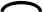
\includegraphics[width=0.1\linewidth]{ellipse0001} &

\includegraphics[width=0.1\linewidth]{ellipse0002} \\
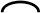
\includegraphics[width=0.1\linewidth]{ellipse0003} &

\includegraphics[width=0.1\linewidth]{ellipse0004} \\

\includegraphics[width=0.1\linewidth]{ellipse0005} &

\includegraphics[width=0.1\linewidth]{ellipse0006} \\
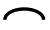
\includegraphics[width=0.1\linewidth]{ellipse0007} &
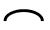
\includegraphics[width=0.1\linewidth]{ellipse0008} \\
%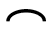
\includegraphics[width=0.1\linewidth]{ellipse0009} & 
%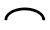
\includegraphics[width=0.1\linewidth]{ellipse0010} \\ 
        \multicolumn{2}{c}{ (a) Data }\\
\end{tabular}
        &
\begin{tabular}{c}
\begin{tabular}{lcr}
\multicolumn{3}{c}{Pearson's r }\\
        -1 & 
\includegraphics[width=0.6\linewidth]{colorbar} & 1
\end{tabular}\\
\begin{tabular}{l|c|c|c}
%\rowcolor{col3}\\ 
        \hline 
Intensity&
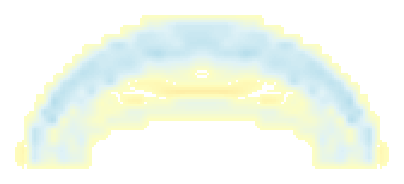
\includegraphics[width=0.18\linewidth]{cor-mass-intensity} &
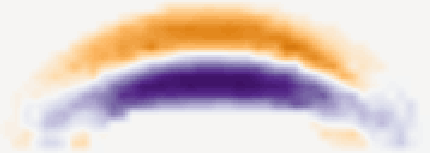
\includegraphics[width=0.18\linewidth]{cor-rx-ry-intensity} &
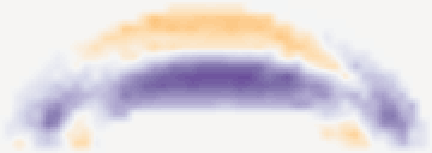
\includegraphics[width=0.18\linewidth]{cor-rx-ry-mass-intensity} \\ \hline
%\rowcolor{col1}
Mass&
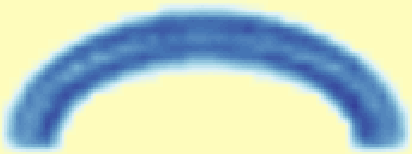
\includegraphics[width=0.18\linewidth]{cor-mass-mass} &
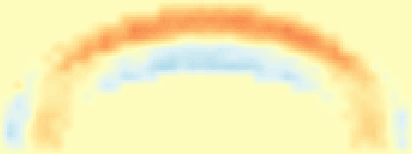
\includegraphics[width=0.18\linewidth]{cor-rx-ry-mass} &
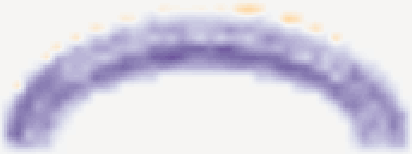
\includegraphics[width=0.18\linewidth]{cor-rx-ry-mass-mass} \\
%\rowcolor{col2}
Cost&
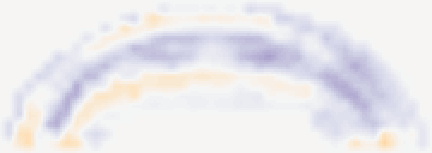
\includegraphics[width=0.18\linewidth]{cor-mass-cost} &
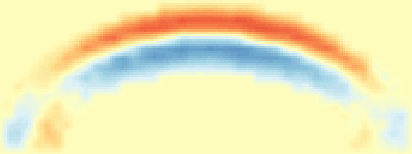
\includegraphics[width=0.18\linewidth]{cor-rx-ry-cost} &
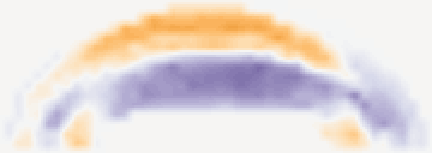
\includegraphics[width=0.18\linewidth]{cor-rx-ry-mass-cost} \\ \hline 
%\rowcolor{white}
        & (b) Size 
        & (c) Shape 
        & (d) Shape + Size 
\end{tabular}
\end{tabular}\\
\end{tabular}
        \\ \hline \hline 
\begin{tabular}{c|c|c}
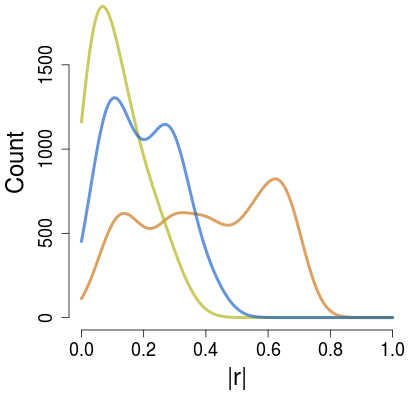
\includegraphics[width=0.3\linewidth]{hist-mass} &
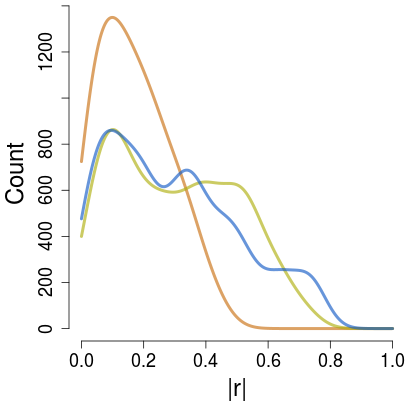
\includegraphics[width=0.3\linewidth]{hist-ellipticity} &
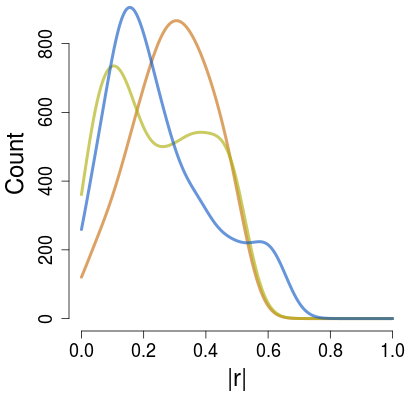
\includegraphics[width=0.3\linewidth]{hist-additive} \\ \hline 
        (e) Size & (f) Shape & (g) Shape + Size
\end{tabular}
\end{tabular}
\caption{\label{fig:cor-ellipse}
Illustration of unbalanced optimal transport on a (a) toy data set of a 100
half ellipses with different minor, major radii and width.  Spatial
correlations of (b) size (number of black pixels), (c) shape (ratio of the
minor and major radii) and (d) sum of size and shape to pixel
intensity values, (middle) mass allocation and (bottom) transport costs.
(f,g,h) Smoothed counts of Pearson's r correlation from the spatial
correlations. The optimal transport approach identifies the changes in size in
the mass imbalance with much stronger correlations than the intensity based
approach.  Shape is captured in both transport cost and intensity, with
slightly stronger correlations with transport cost. Correlation to an additive
shape and mass effect are correctly identified in both transport cost and mass
imbalance, while the intensity values alone lead to weak correlations. The
proposed method correctly identifies shape versus mass effects.  
}
\end{figure}

We demonstrate the proposed method on white and gray matter masks of the OASIS
brain data set~\citep{marcus2010open}. We choose to use the gray and white
matter masks instead of MRI intensity values because of the difficulties in
normalizing the intensities across subjects. However, the method can without
modification be applied to continuous graylevel values or with the definition
of a corresponding cost function even to vector or tensor valued measures. The
only requirement is that the measurement are commensurable across subjects.

\section{Related Work}

Optimal transport and the associated Wasserstein metric, also referred to as
Earth-movers distance, have been extensively used in computer vision
applications. Recent advances that permit fast computation of optimal transport
maps on large data sets lead to a flurry of research in machine learning and 
%Both the mass allocation take into account global effects, in particular the
%shape measures can capture non-local changes, such as
%relative positions of anatomical structures as long as they are no removed
%during the spatial normalization step.  

Voxel-based morphometry (VBM) is a popular approach to detect anatomical
changes by comparing, potentially modulated, intensities at each voxel after
spatial normalization. Similarly Tensor-based morphometry (TBM) compares
measures derived, typically the Jacobian determinant, from a non-linear spatial
normalization that aligns the subjects of the population to a single template
at each voxel. Deformation-based morphometry (DBM) address the issue of finding
global effects but are more difficult to interpret and lack the localization of
the statistical parametric maps (SPM) resulting from voxelwise comparisons.


%VBM
Voxel-based morphometry (VBM) yields spatially localized changes in brain
anatomy but has been shown to be sensitive to mis-registration and is incapable
of discovering globally occurring changes. 
%DBM
Deformation-based morphometry (DBM) takes a more global approach by analysis of
deformation fields. While DBM yields overall measures of changes in shape, the
results are sensitive to the parametrization and regularization of the
deformation field and require delineation of regions of interest to average
deformation field statistics. A priori definition of regions defeats the
purpose of automatic discovery of relevant anatomical changes. 
%Manifold model
The manifold model approach extends DBM to allow for possible non-linear
relationships in the data and avoids having to select a template.
%Visualization
For both approaches visualization of relevant changes is difficult.
%OT map based
In \cite{} propose an optimal transport based approach that is similar to DBM
but uses a optimal transport map parametrization to a template. The approach 
%OT voxel based, this work
The unbalanced optimal transport approach presents a mixture between VBM and
DBM based methods.  While the resulting analysis is voxelwise, the quantities
compared stem from a global optimization problem which mitigates some of the
issues of a traditional VBM and introduces a way that moves towards separating
effects due to changes in volume from effects due to changes in shape.

Optimal transport is not sensitive to small misalignments in the spatial
normalization step which result only in a small transport cost of shifting mass
a short distance. As in VBM the spatial normalization introduces an invariance
to the spatial affect that are normalized, these can be introduced as in VBM by
modulating the mass with the Jacobian determinant to correct for volume changes
otherwise lost in the spatial normalization step. 





\section{Unbalanced Optimal Transport for Population Analysis}
Optimal transport is the problem of minimizing the cost of moving a source
probability distribution to a target probability distribution given a function
that assigns costs to moving mass from source to target locations.   For two
probability measures  $\mu$ and $\nu$ on probability spaces ${\Xsp}$ and
${\Ysp}$ respectively, a coupling of $\mu$ and $\nu$ is a measure $\coupling$
on ${\Xsp}\times{\Ysp}$ such that the marginals of $\coupling$ are $\mu$ and
$\nu$. To define optimal transport and optimal couplings, we need a cost
function $\cost(x,y)$ on ${\Xsp}\times{\Ysp}$ representing the work or cost
needed to move a unit of mass from $x$ to $y$. An optimal coupling $\coupling^*$
minimizes this cost over all choices of couplings $\mathcal{C}(\mu,\nu)$ between
$\mu$ and $\nu$: 
\begin{equation}
\coupling^*=\arg\min_{\coupling\in\mathcal{C}(\mu,\nu)}\left(\int_{{\Xsp}}\int_{{\Xsp}}
\cost(x,y)  d\coupling(x,y)\right)^{\frac1p}\,.  
\end{equation}

For two discrete distributions $\mu = \sum_1^n w(x_i) \delta(x_i)$ and $ \nu =
\sum_1^m v(y_i) \delta(y_i)$ with $\sum w(x_i) = \sum v(y_i) = 1$ the optimal
transport problem is equivalent to the linear program 
\begin{equation}
\min_\coupling \sum_{\substack{i=1,\dots,n\\ j=1,\dots,m}} 
      \cost(x_i, y_j) \coupling(x_i, y_j) \quad \text{s.t.}\quad 
\begin{cases}
\sum_j \coupling(x_i, y_j) = \mu(\{x_i\}) = w(x_i) & \\ 
\sum_i \coupling(x_i, y_j) = \nu(\{y_j\}) = v(y_j) & \\
 \coupling(x_i,y_j)\ge 0
\end{cases}\,.
\label{e:LPformulation}
\end{equation} 
The solution is called an optimal coupling $\coupling^*$, and the minimum value
attained at $\coupling^*$, is called the cost of $\pi^*$, or the optimal cost
of the transport problem, and is denoted by
$\couplingcost(\coupling^*)=\sum_{i,j} \cost(x_i,y_j)\pi^*(x_i,y_j)$. The
constraints enforce that $\coupling$ is a coupling. The variables
$\coupling(x_i, y_j)$ correspond to the amount of mass transported from source
$x_i$ to target $y_j$, at cost $\cost(x_i, y_j)$.

To extend the formulation to deal with arbitrary positive measures $\mu$ and
$\nu$ which do not sum to one the linear program is modified to allow for the
creation of mass. Without loss of generality $\sum_1^n w(x_i)  - \sum_1^m
v(y_i) = \delta \ge 0$, the linear program is modified to allow for the
creation of mass at locations $x_i$ by adding a new source location $z$ and
constraints that amount to adding at most $w(x_i)$ to any location $x_i$ for
free. The linear program reads: 
\begin{equation}
\min_\coupling \sum_{\substack{i=1,\dots,n\\ j=1,\dots,m}} 
      \cost(x_i, y_j) \coupling(x_i, y_j) \quad \text{s.t.}\quad 
\begin{cases}
  \sum_j \coupling(x_i, y_j) + \coupling(z, x_i) = \mu(\{x_i\}) = w(x_i) & \\ 
  \sum_i \coupling(x_i, y_j) = \nu(\{y_j\}) = v(y_j) & \\
  \sum_i \coupling(z, x_i)  = \delta \\
  \coupling(x_i, y_j) \ge 0 \\
  \coupling(z, x_i) \ge 0
\end{cases}\,.
\label{e:LPformulation}
\end{equation} 

This modification results in a standard optimal transport problem through the
addition of target location $z$ that can receive $\delta$ mass at zero cost.
This permits to solve the optimal transport problem with fast approximation
algorithms for large data sets such as the Sinkhorn approach by~\cite{cutuiri:}
or the multiscale strategies by~\citet{gerber:jmlr17}. 


\subsection{Morphometry Pipeline}




\section{Application to OASIS Brain MRI}

The results on the gray matter mask show an increase in the pons area
correlated with CDR and even more so with MMSE.  A hypointense T1 signal in the
pons area has been associated central pontine myelinolysis, which is linked to
alcoholism. The pons in healthy patients typically identified as white matter,
the hypointense signal could potentially lead to a identification with gray
matter, leading to a surplus of gray matter in that area.

\begingroup
\renewcommand{\arraystretch}{0}
\setlength{\tabcolsep}{0pt}
\begin{figure}[bth]
\centering
\begin{tabular}{l|cc|cc|cc} 
\parbox[t]{4mm}{\multirow{3}{*}{\rotatebox[origin=c]{90}{Mass Imbalance}}}&
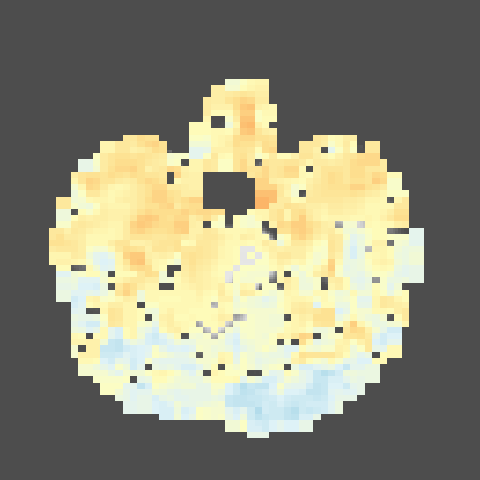
\includegraphics[width=0.16\linewidth]{cor-axial-age-mW} &
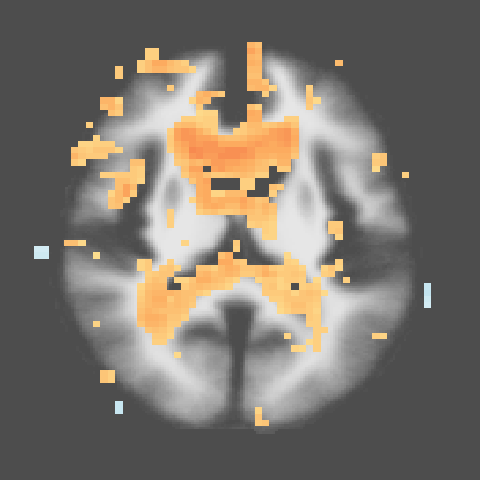
\includegraphics[width=0.16\linewidth]{cor-axial-age-t-mW} &
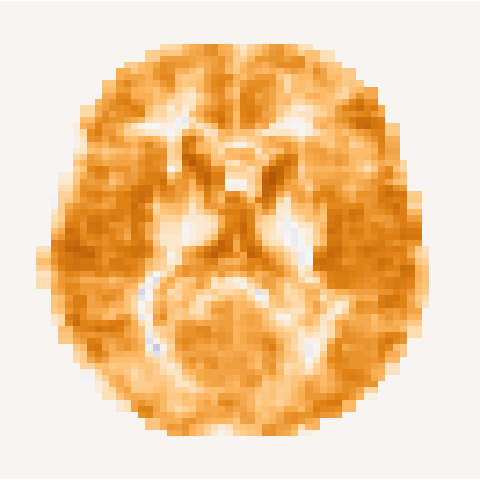
\includegraphics[width=0.16\linewidth]{cor-axial-cdr-mW} &
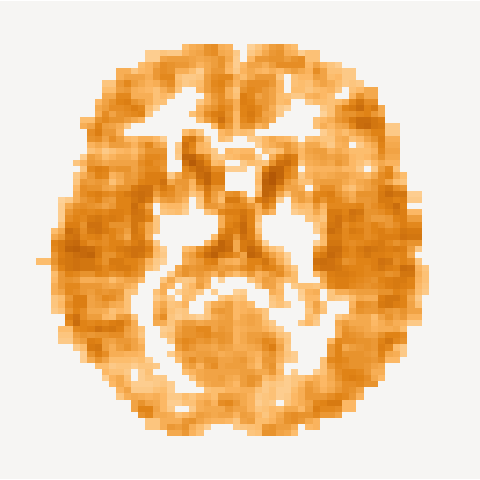
\includegraphics[width=0.16\linewidth]{cor-axial-cdr-t-mW} &
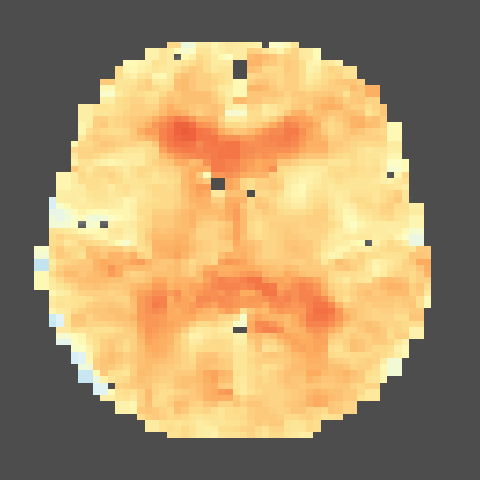
\includegraphics[width=0.16\linewidth]{cor-axial-mmse-mW} &
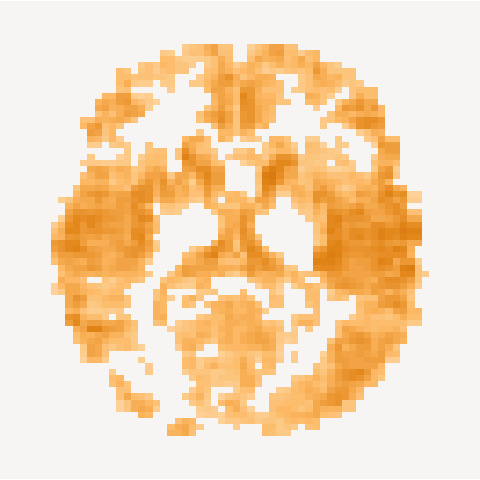
\includegraphics[width=0.16\linewidth]{cor-axial-mmse-t-mW} \\ 
%
        &
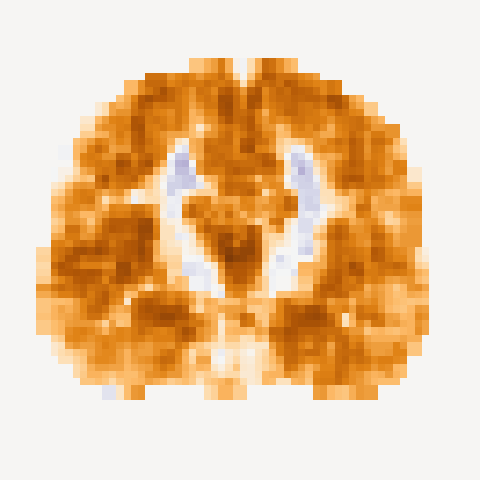
\includegraphics[width=0.16\linewidth]{cor-coronal-age-mW} &
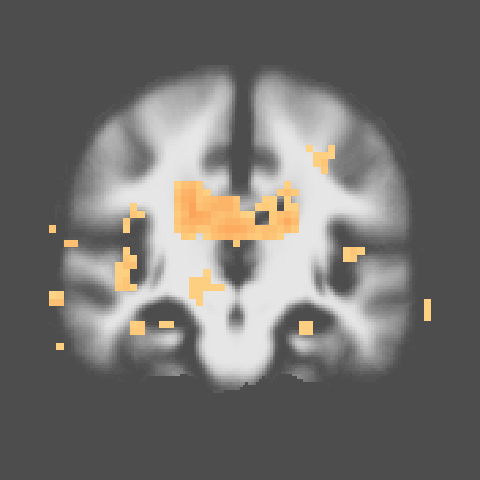
\includegraphics[width=0.16\linewidth]{cor-coronal-age-t-mW} &
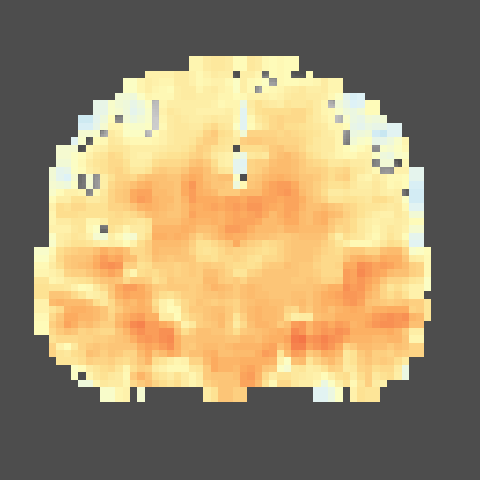
\includegraphics[width=0.16\linewidth]{cor-coronal-cdr-mW} &
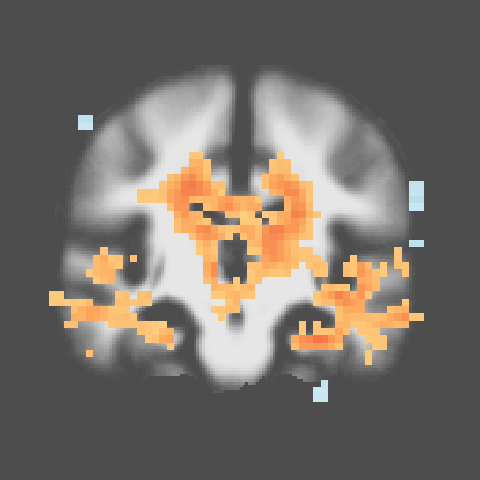
\includegraphics[width=0.16\linewidth]{cor-coronal-cdr-t-mW} &
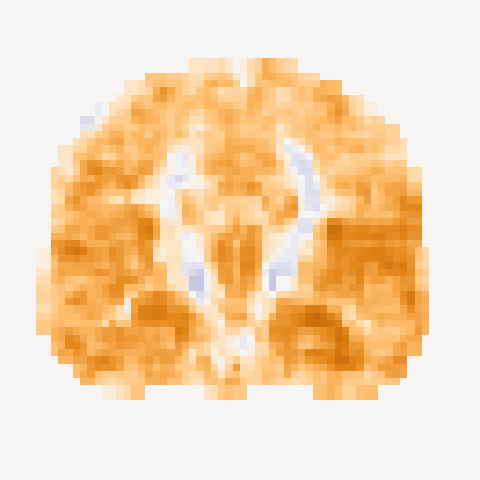
\includegraphics[width=0.16\linewidth]{cor-coronal-mmse-mW} &
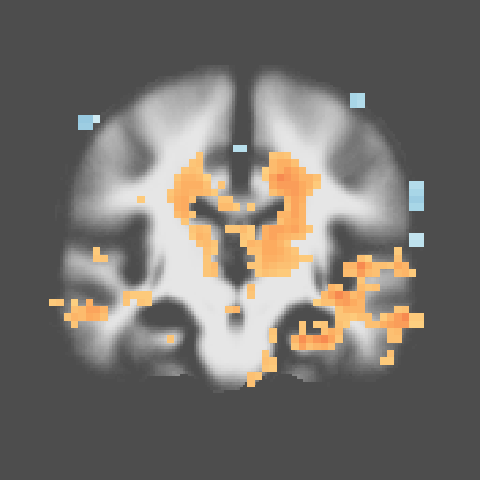
\includegraphics[width=0.16\linewidth]{cor-coronal-mmse-t-mW} \\ 
%
        &
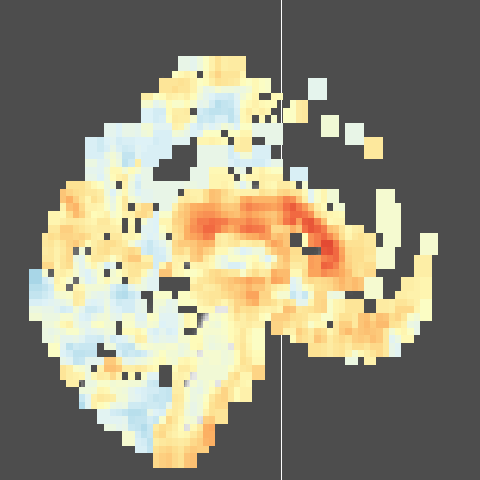
\includegraphics[width=0.16\linewidth]{cor-sagital-age-mW} &
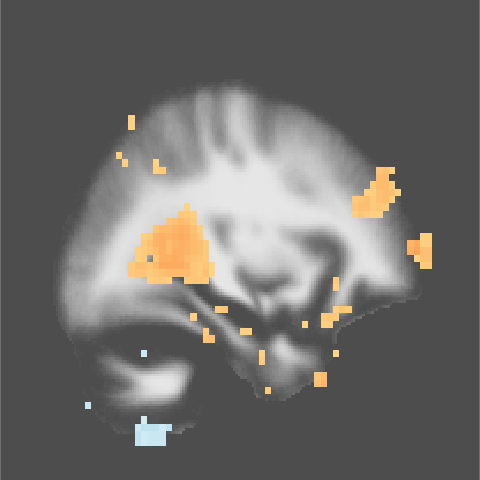
\includegraphics[width=0.16\linewidth]{cor-sagital-age-t-mW} &
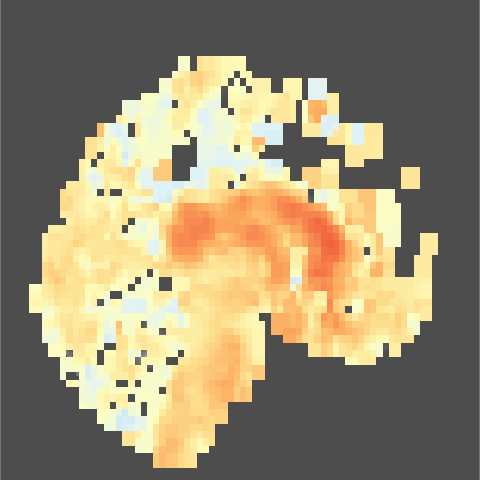
\includegraphics[width=0.16\linewidth]{cor-sagital-cdr-mW} &
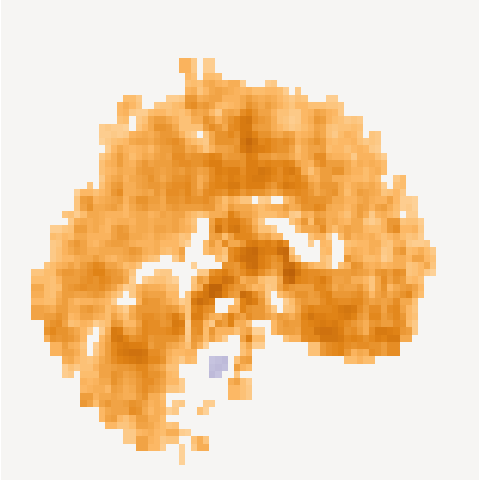
\includegraphics[width=0.16\linewidth]{cor-sagital-cdr-t-mW} &
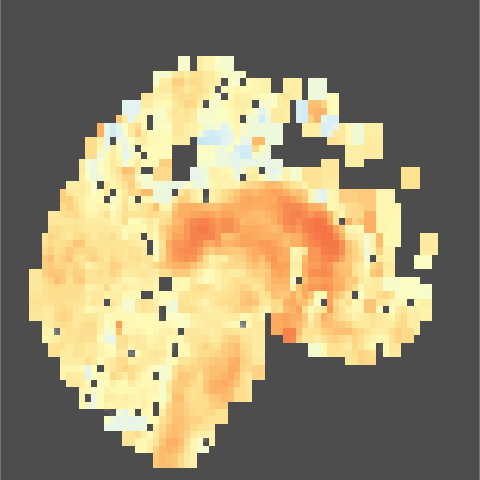
\includegraphics[width=0.16\linewidth]{cor-sagital-mmse-mW} &
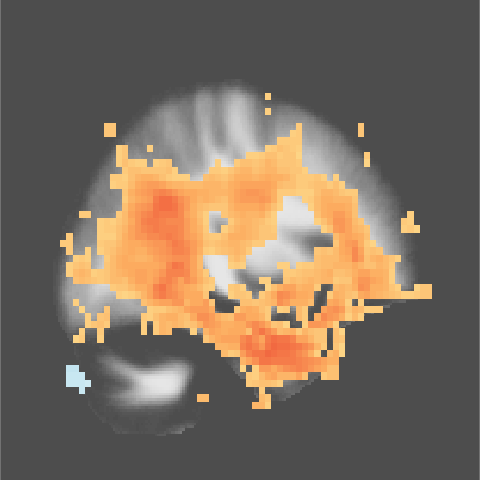
\includegraphics[width=0.16\linewidth]{cor-sagital-mmse-t-mW} \\ \hline \hline
%
\parbox[t]{2mm}{\multirow{3}{*}{\rotatebox[origin=c]{90}{Transport Cost}}}&
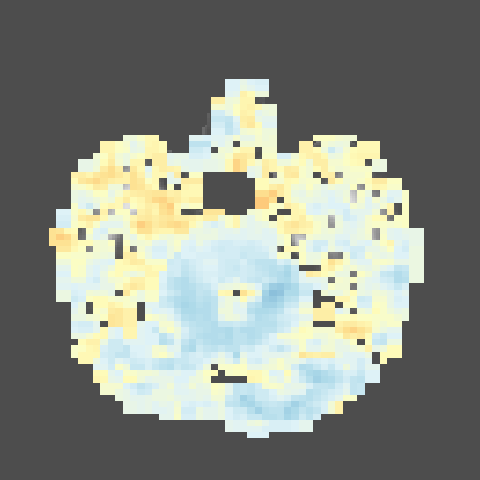
\includegraphics[width=0.16\linewidth]{cor-axial-age-tW} &
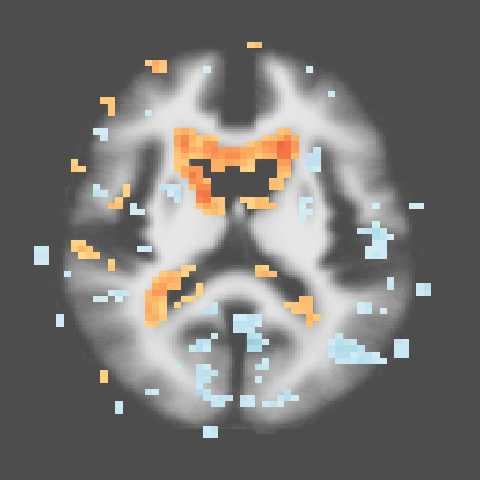
\includegraphics[width=0.16\linewidth]{cor-axial-age-t-tW} &
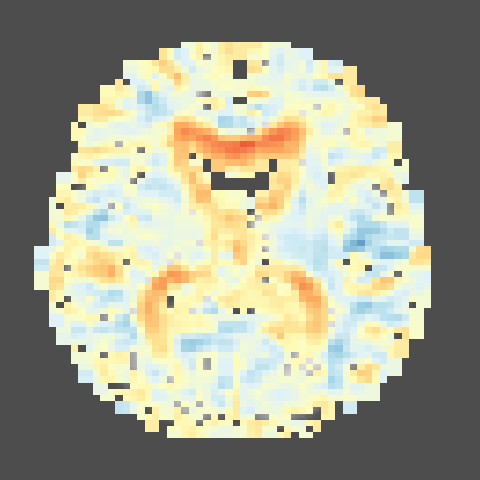
\includegraphics[width=0.16\linewidth]{cor-axial-cdr-tW} &
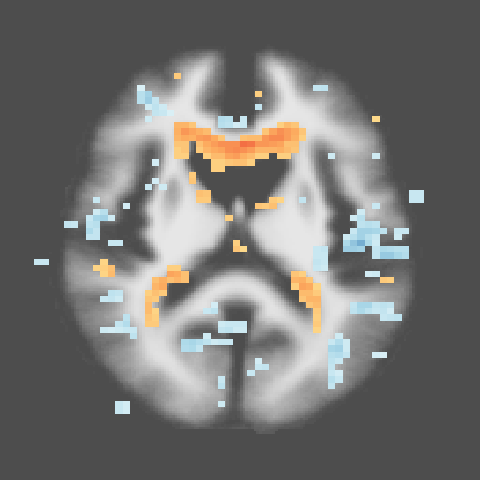
\includegraphics[width=0.16\linewidth]{cor-axial-cdr-t-tW} &
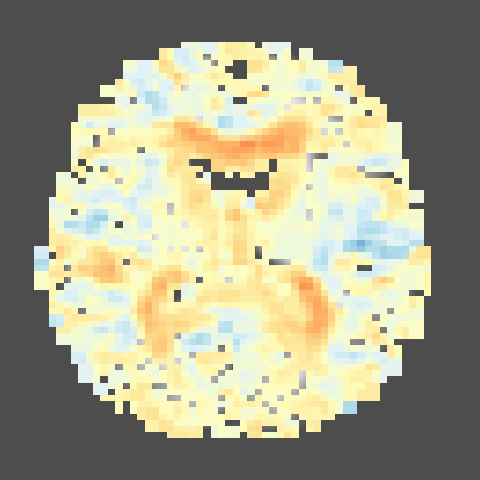
\includegraphics[width=0.16\linewidth]{cor-axial-mmse-tW} &
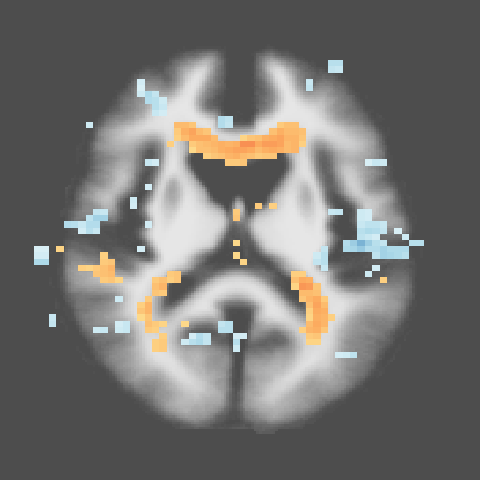
\includegraphics[width=0.16\linewidth]{cor-axial-mmse-t-tW} \\ 
%
        &
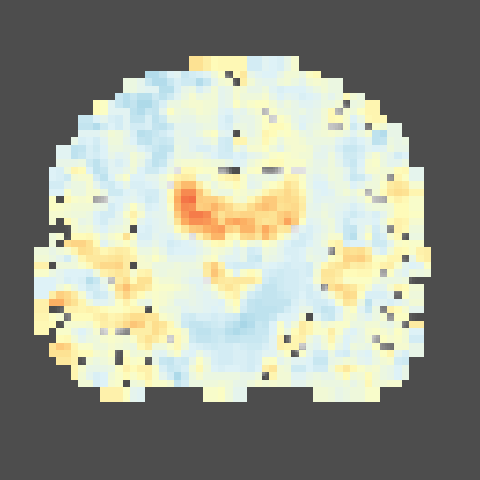
\includegraphics[width=0.16\linewidth]{cor-coronal-age-tW} &
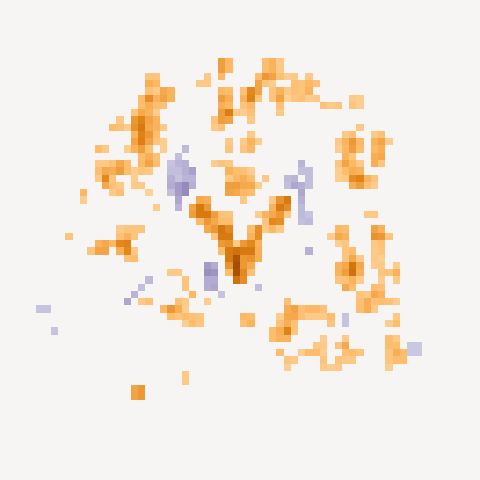
\includegraphics[width=0.16\linewidth]{cor-coronal-age-t-tW} &
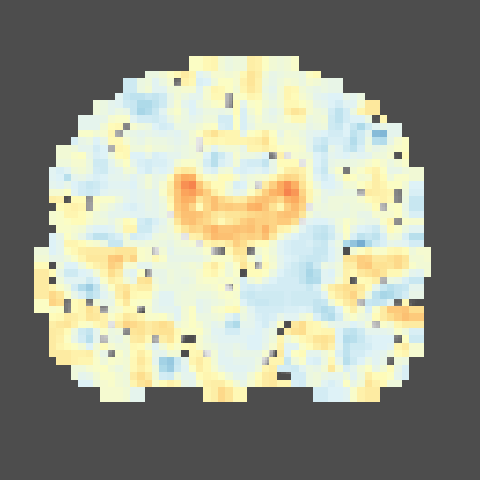
\includegraphics[width=0.16\linewidth]{cor-coronal-cdr-tW} &
\includegraphics[width=0.16\linewidth]{cor-coronal-cdr-t-tW} &
\includegraphics[width=0.16\linewidth]{cor-coronal-mmse-tW} &
\includegraphics[width=0.16\linewidth]{cor-coronal-mmse-t-tW} \\ 
%
        &
\includegraphics[width=0.16\linewidth]{cor-sagital-age-tW} &
\includegraphics[width=0.16\linewidth]{cor-sagital-age-t-tW} &
\includegraphics[width=0.16\linewidth]{cor-sagital-cdr-tW} &
\includegraphics[width=0.16\linewidth]{cor-sagital-cdr-t-tW} &
\includegraphics[width=0.16\linewidth]{cor-sagital-mmse-tW} &
\includegraphics[width=0.16\linewidth]{cor-sagital-mmse-t-tW} \\ \hline \hline
%
& \parbox[b][4mm]{6mm}{Age} 
& \parbox[b][4mm]{6mm}{Age\textsuperscript{*}} 
& \parbox[b][4mm]{6mm}{CDR} 
& \parbox[b][4mm]{6mm}{CDR\textsuperscript{*}}
& \parbox[b][4mm]{6mm}{MMSE}
& \parbox[b][4mm]{6mm}{MMSE\textsuperscript{*}}
\end{tabular}
\caption{\label{fig:cor-oasis-gray}
Correlation of age, MMSE and CDR with optimal transport mass imbalances and
optimal transport costs of gray matter. The columns with a \textsuperscript{*}
only show the voxels were the correlation has a permutation tested p-value less
than 0.05  }
\end{figure}
\endgroup

\begingroup
\renewcommand{\arraystretch}{0}
\setlength{\tabcolsep}{0pt}
\begin{figure}[bth]
\centering
\begin{tabular}{l|cc|cc|cc}
\parbox[t]{4mm}{\multirow{3}{*}{\rotatebox[origin=c]{90}{Mass Imbalance}}}&
\includegraphics[width=0.16\linewidth]{cor-axial-age-mG} &
\includegraphics[width=0.16\linewidth]{cor-axial-age-t-mG} &
\includegraphics[width=0.16\linewidth]{cor-axial-cdr-mG} &
\includegraphics[width=0.16\linewidth]{cor-axial-cdr-t-mG} &
\includegraphics[width=0.16\linewidth]{cor-axial-mmse-mG} &
\includegraphics[width=0.16\linewidth]{cor-axial-mmse-t-mG} \\ 
%
        &
\includegraphics[width=0.16\linewidth]{cor-coronal-age-mG} &
\includegraphics[width=0.16\linewidth]{cor-coronal-age-t-mG} &
\includegraphics[width=0.16\linewidth]{cor-coronal-cdr-mG} &
\includegraphics[width=0.16\linewidth]{cor-coronal-cdr-t-mG} &
\includegraphics[width=0.16\linewidth]{cor-coronal-mmse-mG} &
\includegraphics[width=0.16\linewidth]{cor-coronal-mmse-t-mG} \\ 
%
        &
\includegraphics[width=0.16\linewidth]{cor-sagital-age-mG} &
\includegraphics[width=0.16\linewidth]{cor-sagital-age-t-mG} &
\includegraphics[width=0.16\linewidth]{cor-sagital-cdr-mG} &
\includegraphics[width=0.16\linewidth]{cor-sagital-cdr-t-mG} &
\includegraphics[width=0.16\linewidth]{cor-sagital-mmse-mG} &
\includegraphics[width=0.16\linewidth]{cor-sagital-mmse-t-mG} \\ \hline \hline
%
\parbox[t]{2mm}{\multirow{3}{*}{\rotatebox[origin=c]{90}{Transport Cost}}}&
\includegraphics[width=0.16\linewidth]{cor-axial-age-tG} &
\includegraphics[width=0.16\linewidth]{cor-axial-age-t-tG} &
\includegraphics[width=0.16\linewidth]{cor-axial-cdr-tG} &
\includegraphics[width=0.16\linewidth]{cor-axial-cdr-t-tG} &
\includegraphics[width=0.16\linewidth]{cor-axial-mmse-tG} &
\includegraphics[width=0.16\linewidth]{cor-axial-mmse-t-tG} \\ 
%
        &
\includegraphics[width=0.16\linewidth]{cor-coronal-age-tG} &
\includegraphics[width=0.16\linewidth]{cor-coronal-age-t-tG} &
\includegraphics[width=0.16\linewidth]{cor-coronal-cdr-tG} &
\includegraphics[width=0.16\linewidth]{cor-coronal-cdr-t-tG} &
\includegraphics[width=0.16\linewidth]{cor-coronal-mmse-tG} &
\includegraphics[width=0.16\linewidth]{cor-coronal-mmse-t-tG} \\ 
%
        &
\includegraphics[width=0.16\linewidth]{cor-sagital-age-tG} &
\includegraphics[width=0.16\linewidth]{cor-sagital-age-t-tG} &
\includegraphics[width=0.16\linewidth]{cor-sagital-cdr-tG} &
\includegraphics[width=0.16\linewidth]{cor-sagital-cdr-t-tG} &
\includegraphics[width=0.16\linewidth]{cor-sagital-mmse-tG} &
\includegraphics[width=0.16\linewidth]{cor-sagital-mmse-t-tG} \\ \hline \hline
%%
& \parbox[b][4mm]{6mm}{Age} 
& \parbox[b][4mm]{6mm}{Age\textsuperscript{*}} 
& \parbox[b][4mm]{6mm}{CDR} 
& \parbox[b][4mm]{6mm}{CDR\textsuperscript{*}}
& \parbox[b][4mm]{6mm}{MMSE}
& \parbox[b][4mm]{6mm}{MMSE\textsuperscript{*}}
\end{tabular}
\caption{\label{fig:cor-oasis-white}
Correlation of age, MMSE and CDR with optimal transport mass imbalances and
optimal transport costs of white matter. The columns with a \textsuperscript{*}
only show the voxels were the correlation has a permutation tested p-value less
than 0.05  }
\end{figure}
\endgroup




\section{Conclusion}

Unablanced optimal transport is not restricted to be applied to segmentation
mask, it can be directly applied to graylevel intensities or with an
appropriate cost function to diffusion tensors. 


Combining unbalanced optimal transport with a more globally sensitive analysis.
I.e. the resulting maps are still voxelwise and should be brought into some
correspondence or averaged.

Localized mass preserving

Additional analysis methods: Clustering

\bibliographystyle{apalike}
\bibliography{bot.bib,optimal-transport}


\end{document}
